
\section{Langkah-Langkah Percobaan}

\subsection{Wireless Point to Point}
\begin{enumerate}
    \item Sambungkan kabel LAN dari laptop ke router A, lalu hubungkan router A ke router B.
    \item Akses router melalui Winbox menggunakan MAC address dan lakukan reset konfigurasi ke pengaturan awal.
      \begin{figure}[H]
        \centering
        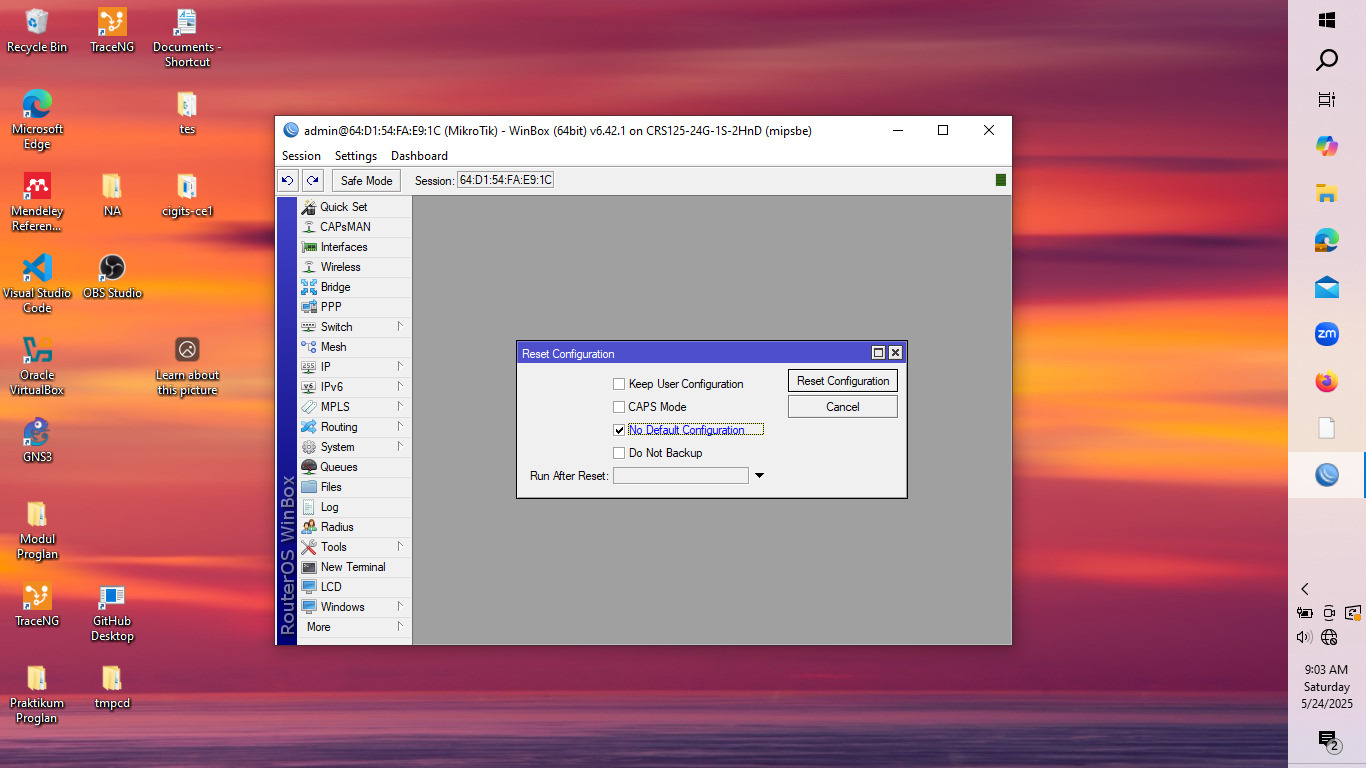
\includegraphics[width=0.5\linewidth]{P1/img/1.jpeg}
        \caption{Reset Configuration}
        \label{fig:gambar4}
    \end{figure}
    \item Aktifkan interface \texttt{wlan1} pada menu Wireless. Atur mode menjadi \textbf{bridge} dan beri SSID \texttt{PointToPoint\_16}.
     \begin{figure}[H]
        \centering
        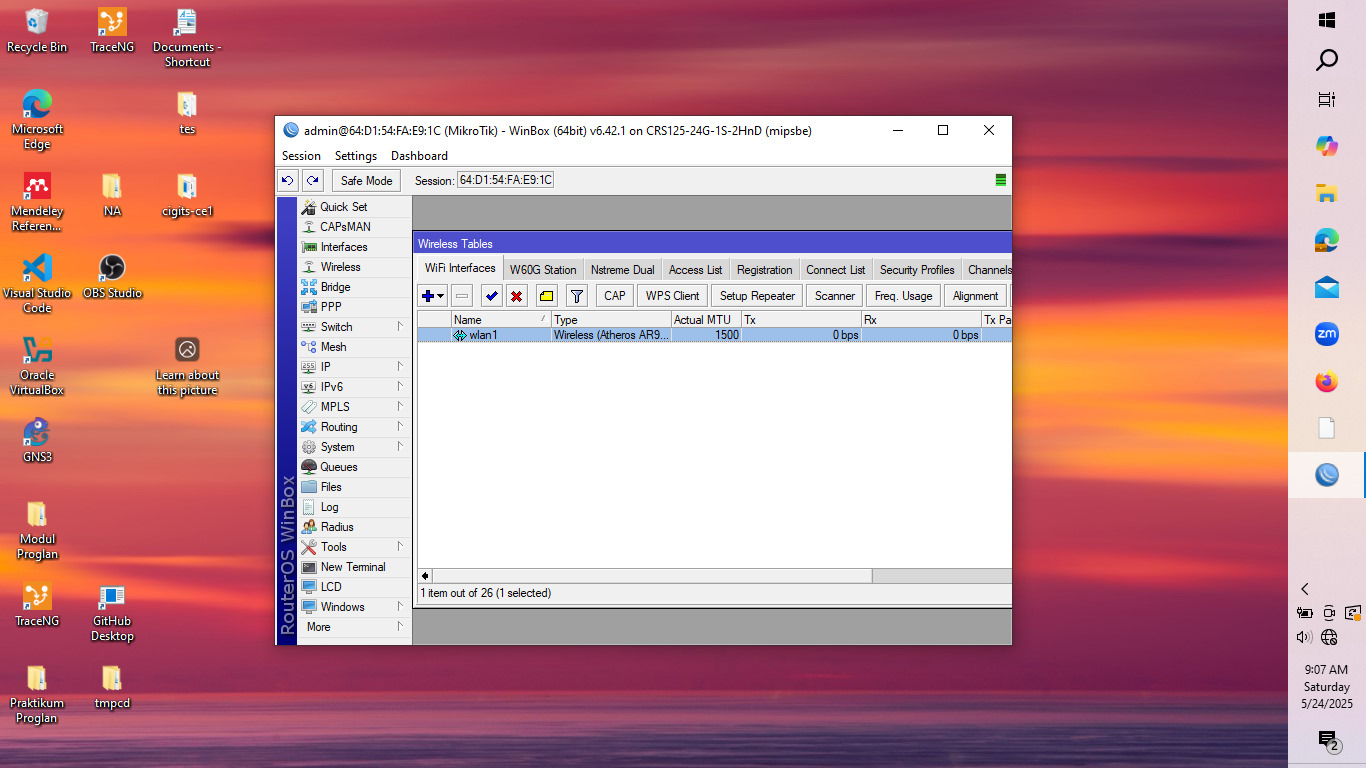
\includegraphics[width=0.5\linewidth]{P1/img/3.jpeg}
        \caption{Aktifkan interface}
        \label{fig:gambar4}
    \end{figure}
    \item Pada router B, aktifkan \texttt{wlan1} dan ubah modenya menjadi \textbf{station}. Klik tombol
    \textit{Scan}, pilih SSID dari router A, lalu tekan \textit{Connect}.
     \begin{figure}[H]
        \centering
        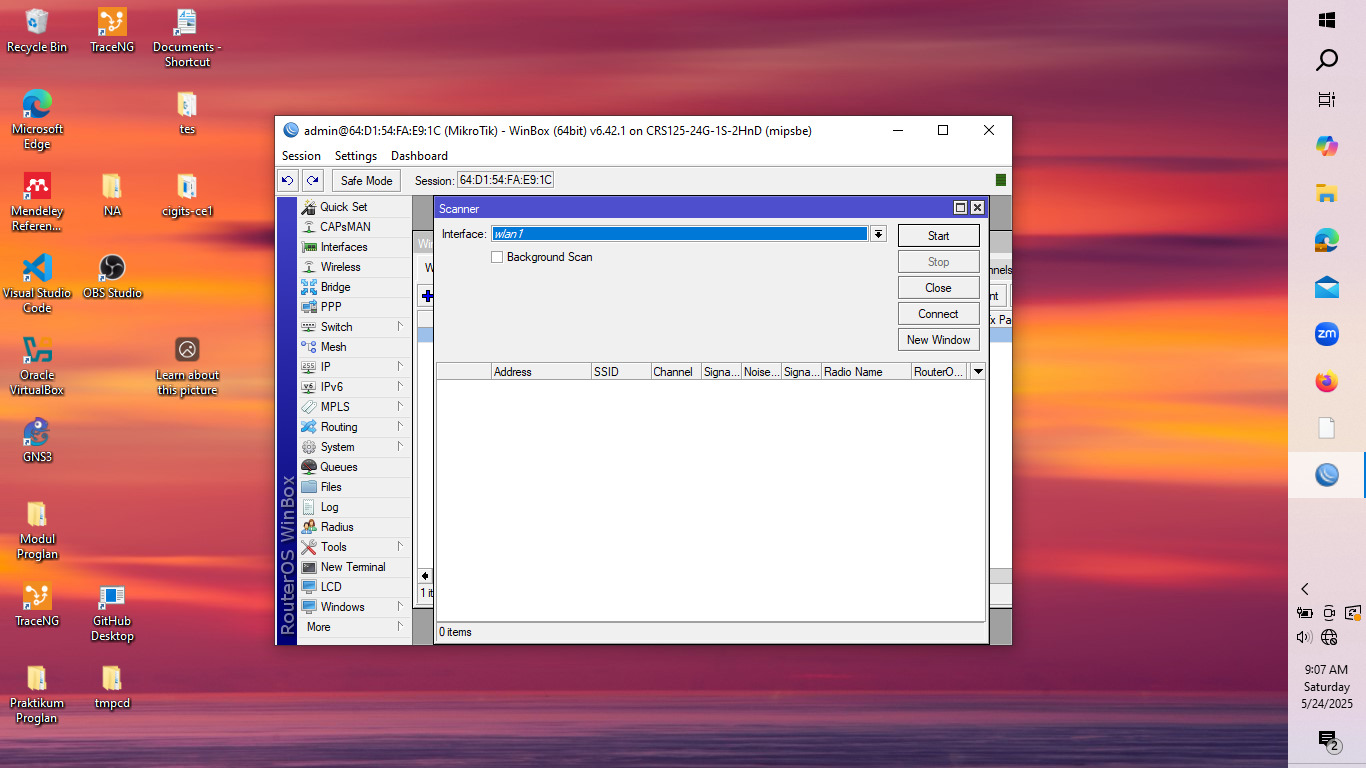
\includegraphics[width=0.5\linewidth]{P1/img/4.jpeg}
        \caption{Aktifkan wlan 1, ubah modenya menjadi station}
        \label{fig:gambar4}
    \end{figure}
    \item Hubungkan Laptop B ke SSID \texttt{PointToPoint\_16} yang dipancarkan Router A.
     \begin{figure}[H]
        \centering
        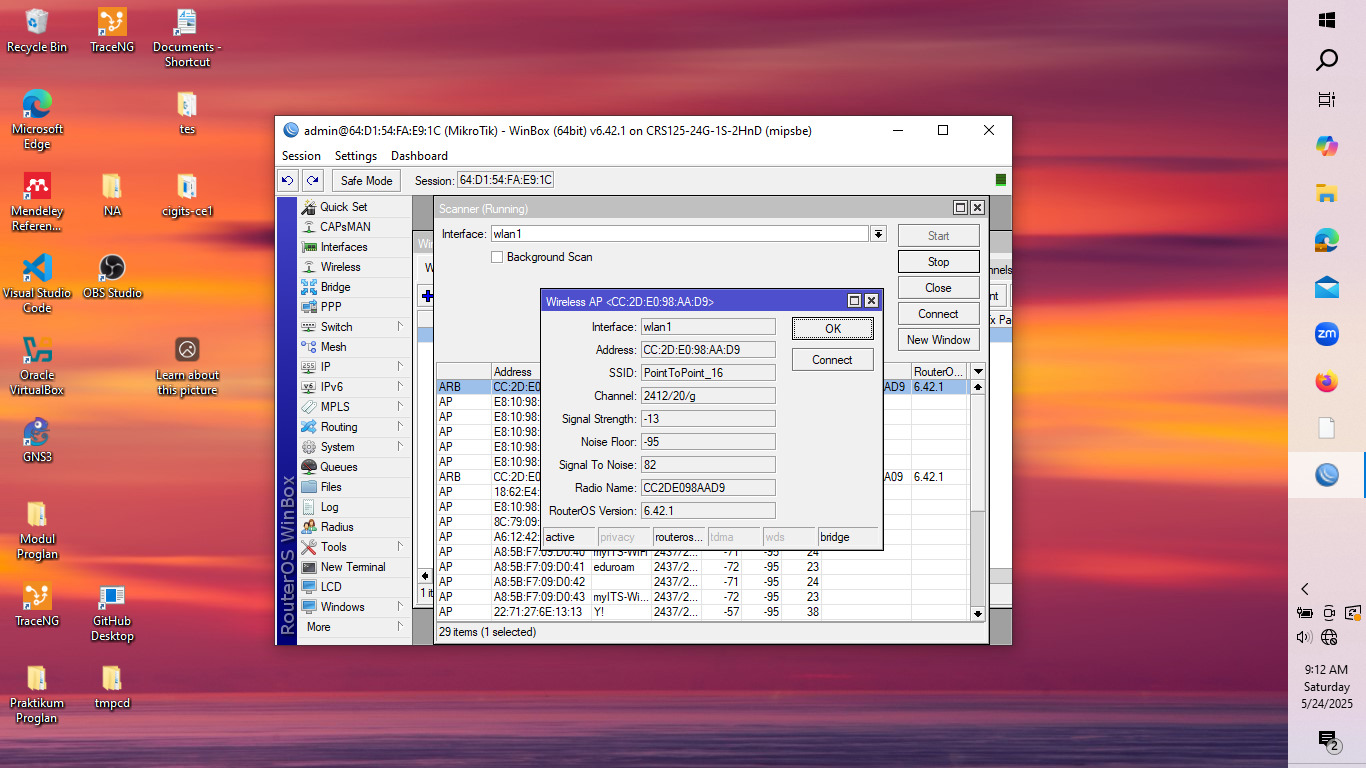
\includegraphics[width=0.5\linewidth]{P1/img/5.jpeg}
        \caption{Hubungkan ke SSID}
        \label{fig:gambar4}
    \end{figure}
    \item Atur IP statis masing-masing laptop sesuai dengan jaringan LAN yang terhubung.
     \begin{figure}[H]
        \centering
        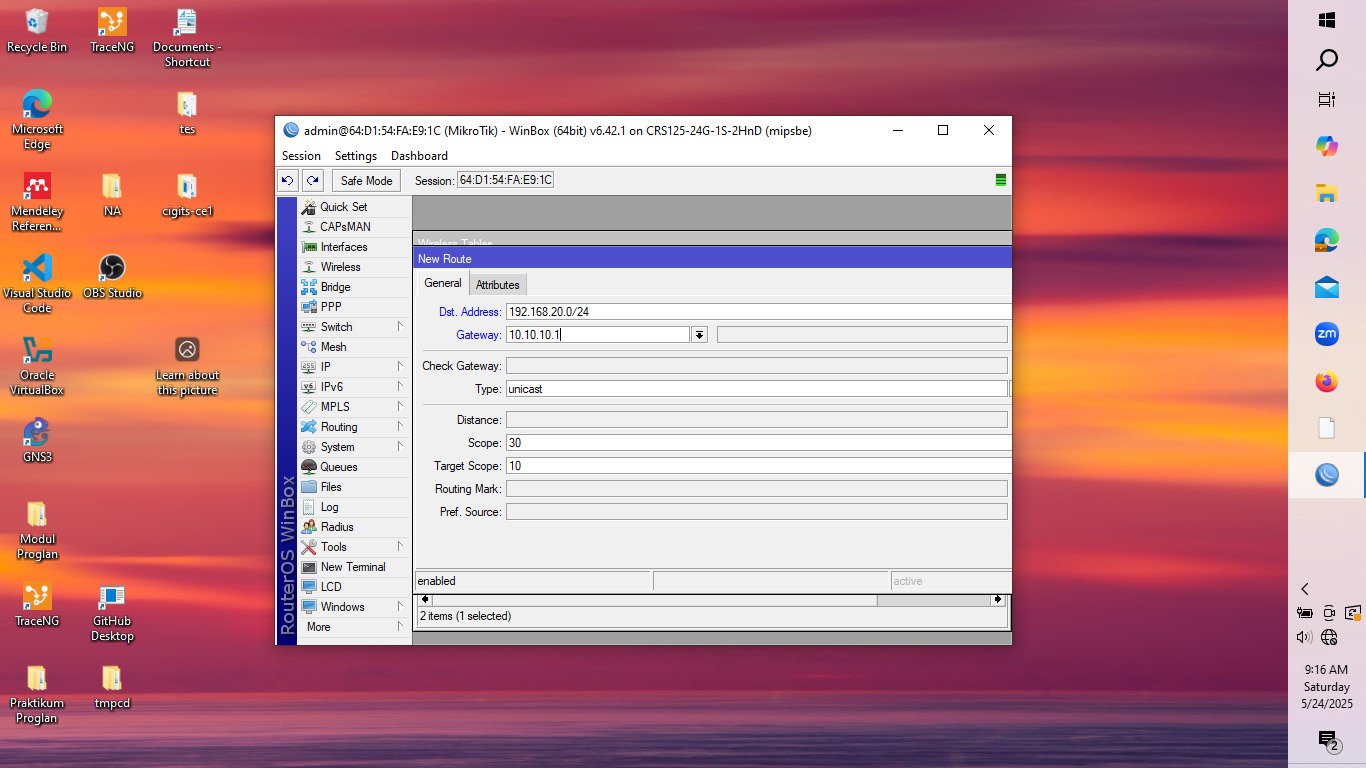
\includegraphics[width=0.5\linewidth]{P1/img/7.jpeg}
        \caption{Atur IP}
        \label{fig:gambar4}
    \end{figure}
    \item Lakukan pengujian koneksi antar laptop menggunakan perintah \texttt{ping}.
     \begin{figure}[H]
        \centering
        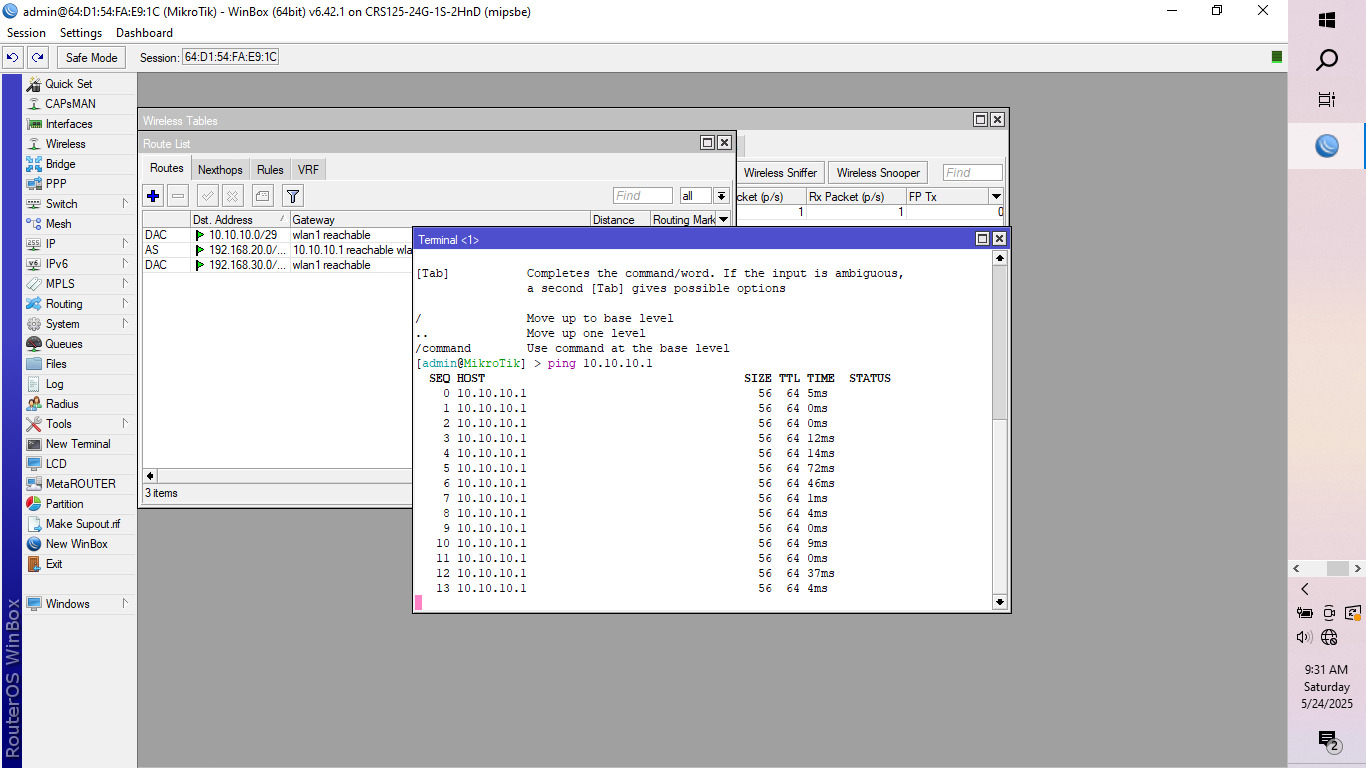
\includegraphics[width=0.5\linewidth]{P1/img/8.jpeg}
        \caption{Lakukan Uji Ping}
        \label{fig:gambar4}
    \end{figure}

\end{enumerate}

\subsection{Wireless Point to Multipoint}
\begin{enumerate}
    \item Sambungkan kabel LAN dari laptop ke router, dan antar router jika diperlukan.
    \item Login ke router menggunakan Winbox dan reset konfigurasi jika masih terdapat pengaturan sebelumnya.
    \begin{figure}[H]
        \centering
        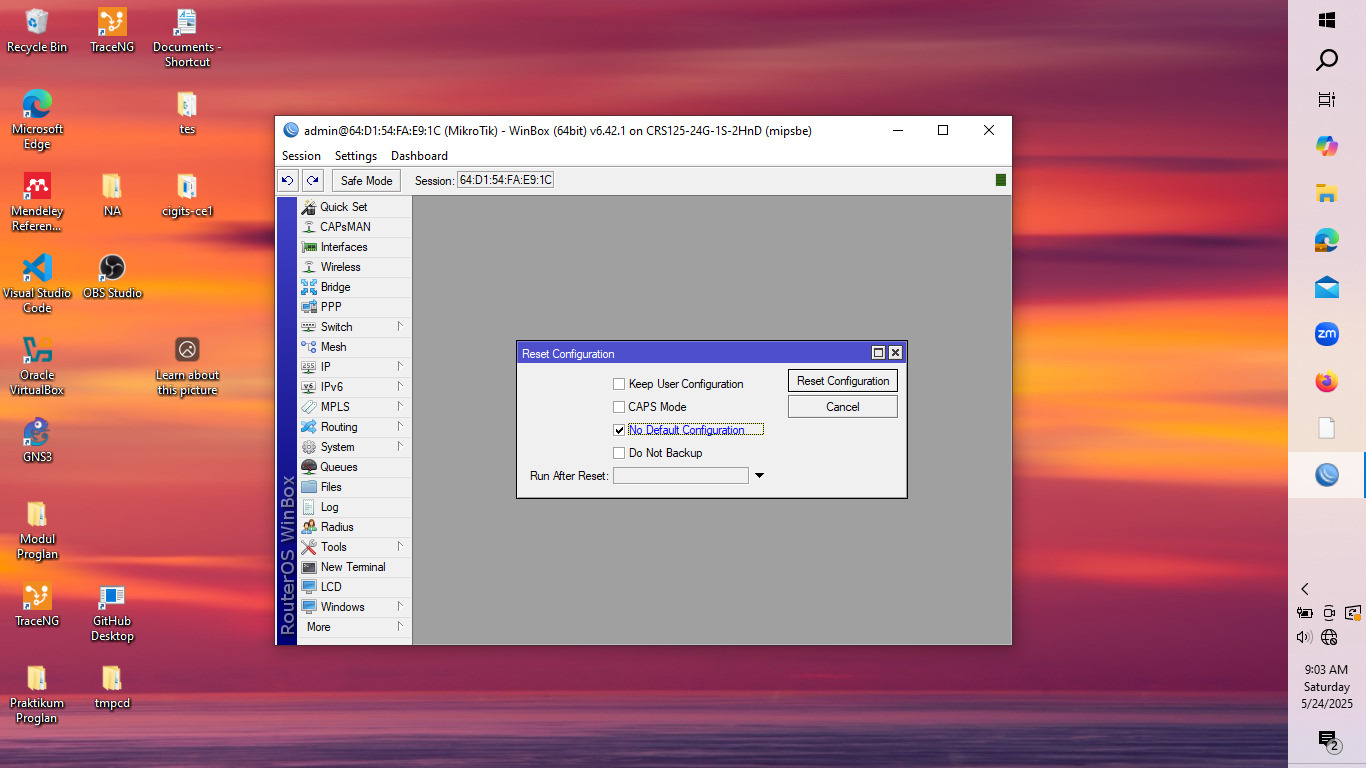
\includegraphics[width=0.5\linewidth]{P1/img/1.jpeg}
        \caption{Reset Configuration}
        \label{fig:gambar4}
    \end{figure}
    \item Aktifkan \texttt{wlan1} pada Router A, ubah mode menjadi \textbf{AP bridge}, dan atur SSID menjadi \texttt{PointToMultiPoint\_16}.
    \begin{figure}[H]
        \centering
        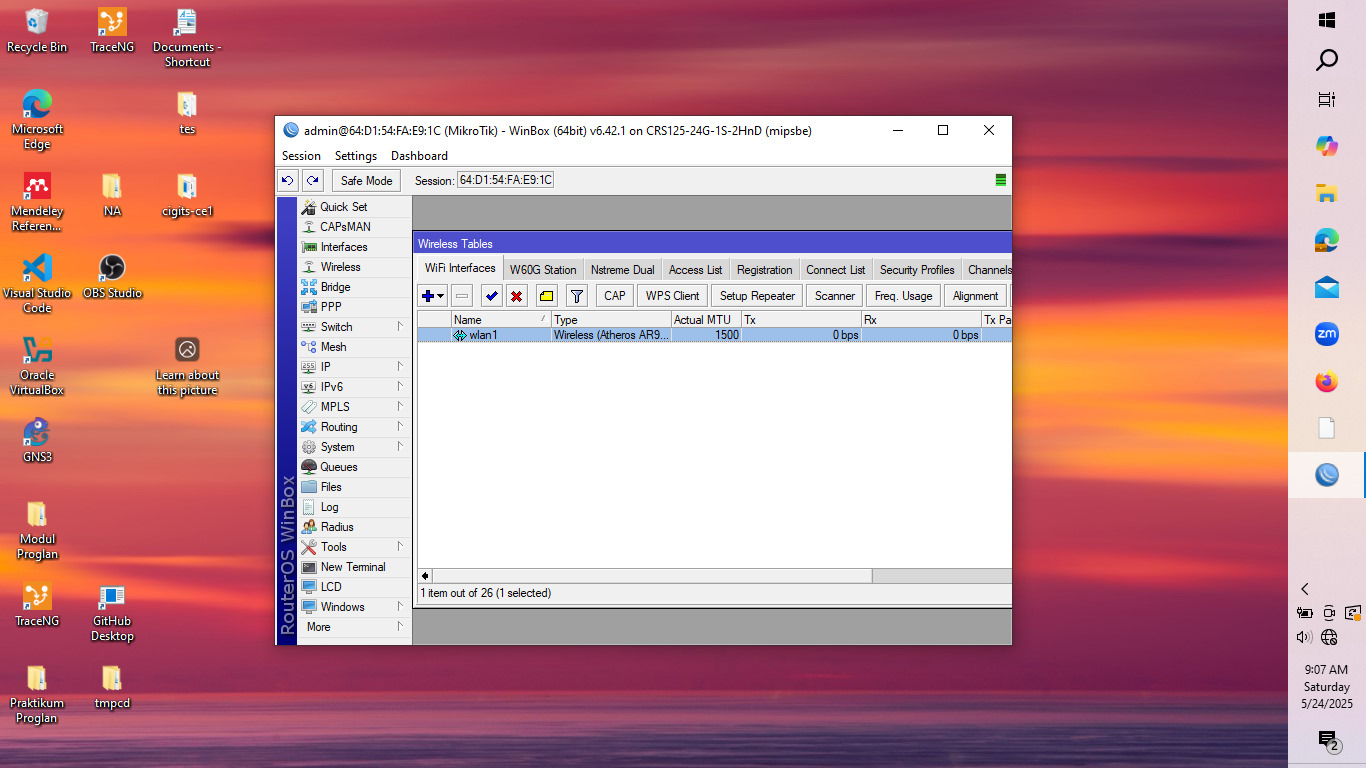
\includegraphics[width=0.5\linewidth]{P1/img/3.jpeg}
        \caption{Aktifkan interface}
        \label{fig:gambar4}
    \end{figure}
    \item Di Router B, aktifkan \texttt{wlan1} lalu ubah ke mode \textbf{station bridge}. Gunakan tombol \textit{Scan} untuk mencari dan menyambung ke SSID dari Router A.
    \begin{figure}[H]
        \centering
        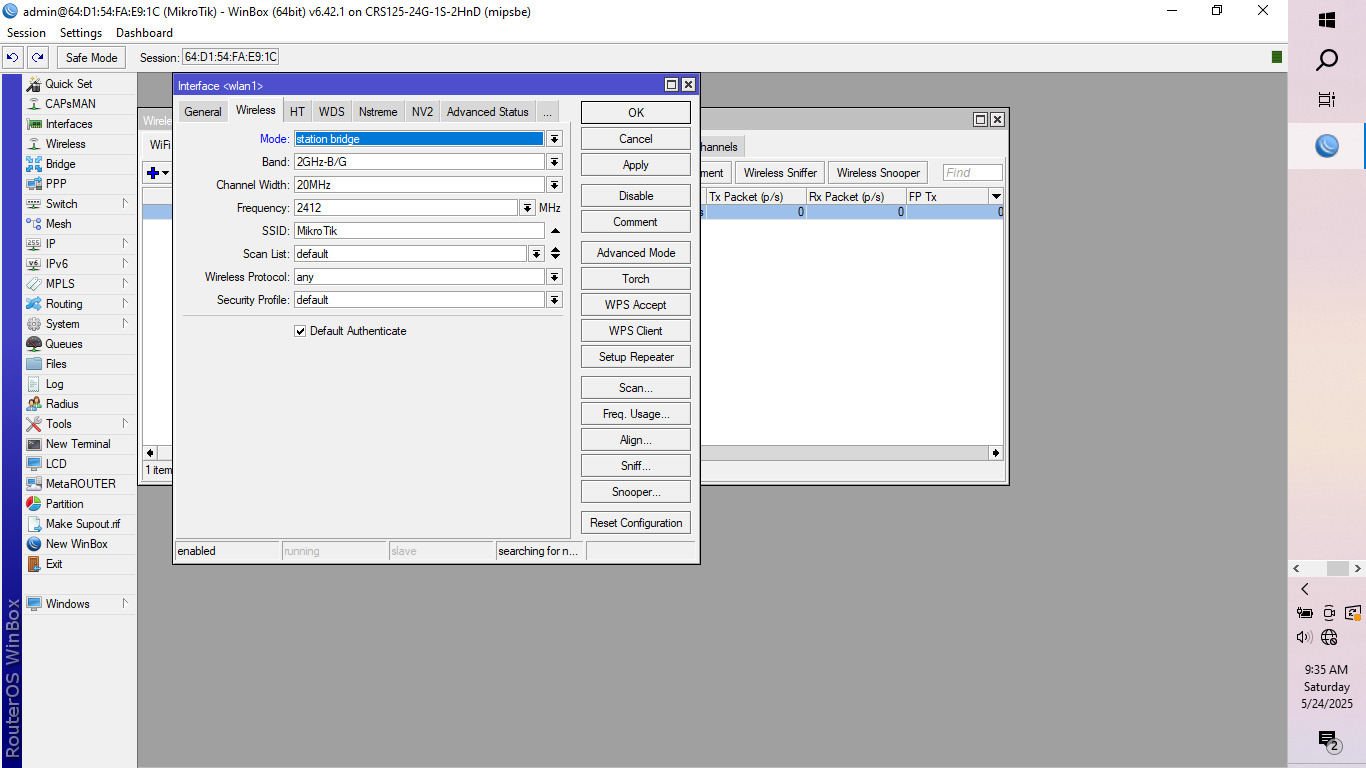
\includegraphics[width=0.5\linewidth]{P1/img/11.jpeg}
        \caption{Aktifkan wlan 1, ubah modenya menjadi Bridge}
        \label{fig:gambar4}
    \end{figure}
    \item Tambahkan alamat IP pada interface \texttt{wlan1} dan \texttt{ether2} di masing-masing router.
    \begin{figure}[H]
        \centering
        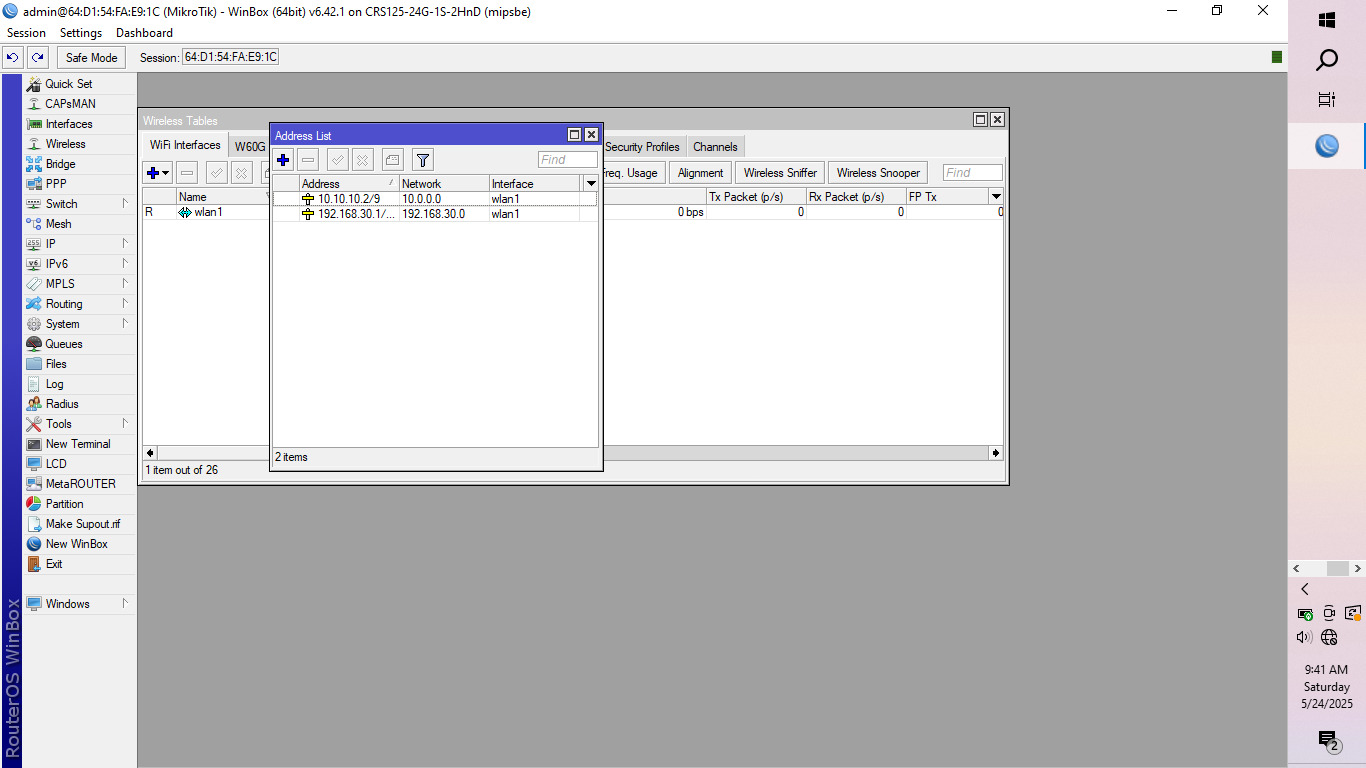
\includegraphics[width=0.5\linewidth]{P1/img/14.jpeg}
        \caption{Tambahkan Alamat IP}
        \label{fig:gambar4}
    \end{figure}
    \item Konfigurasikan routing statis di kedua router agar paket data dapat saling terhubung.
     \begin{figure}[H]
        \centering
        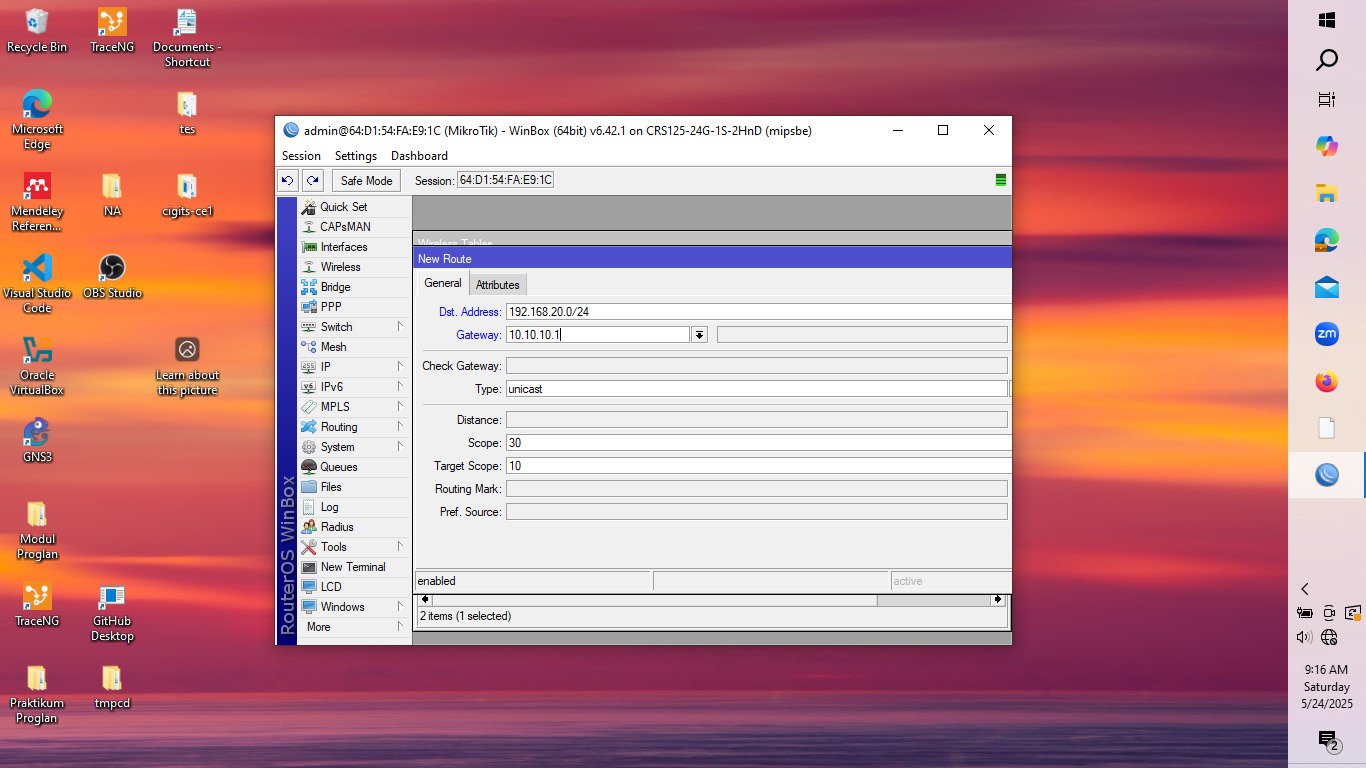
\includegraphics[width=0.5\linewidth]{P1/img/7.jpeg}
        \caption{Konfigurasi Routing}
        \label{fig:gambar4}
    \end{figure}
    \item Atur IP statis di masing-masing laptop melalui \textit{Control Panel} atau pengaturan jaringan.
     \begin{figure}[H]
        \centering
        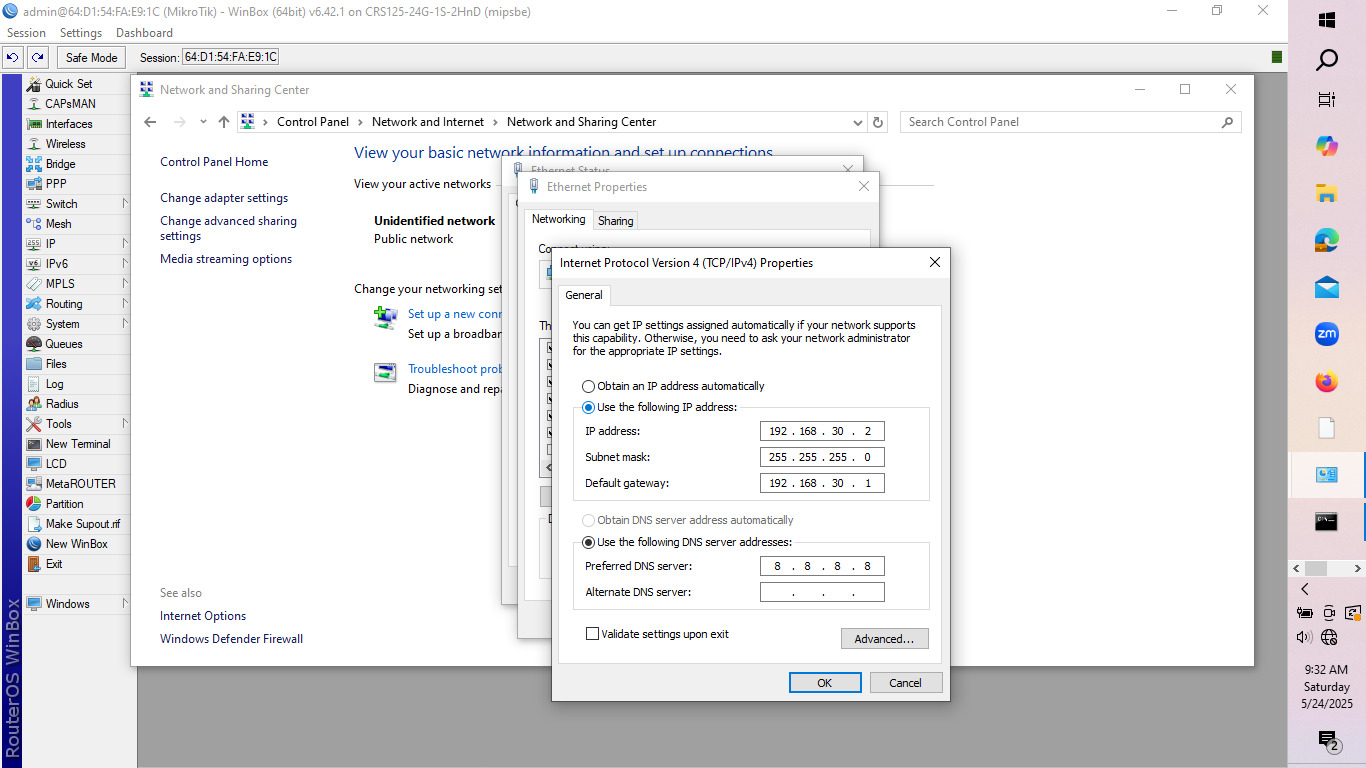
\includegraphics[width=0.5\linewidth]{P1/img/9.jpeg}
        \caption{Atur IP}
        \label{fig:gambar4}
    \end{figure}
    \item Uji koneksi dengan melakukan \texttt{ping} dari satu laptop ke laptop lain.
     \begin{figure}[H]
        \centering
        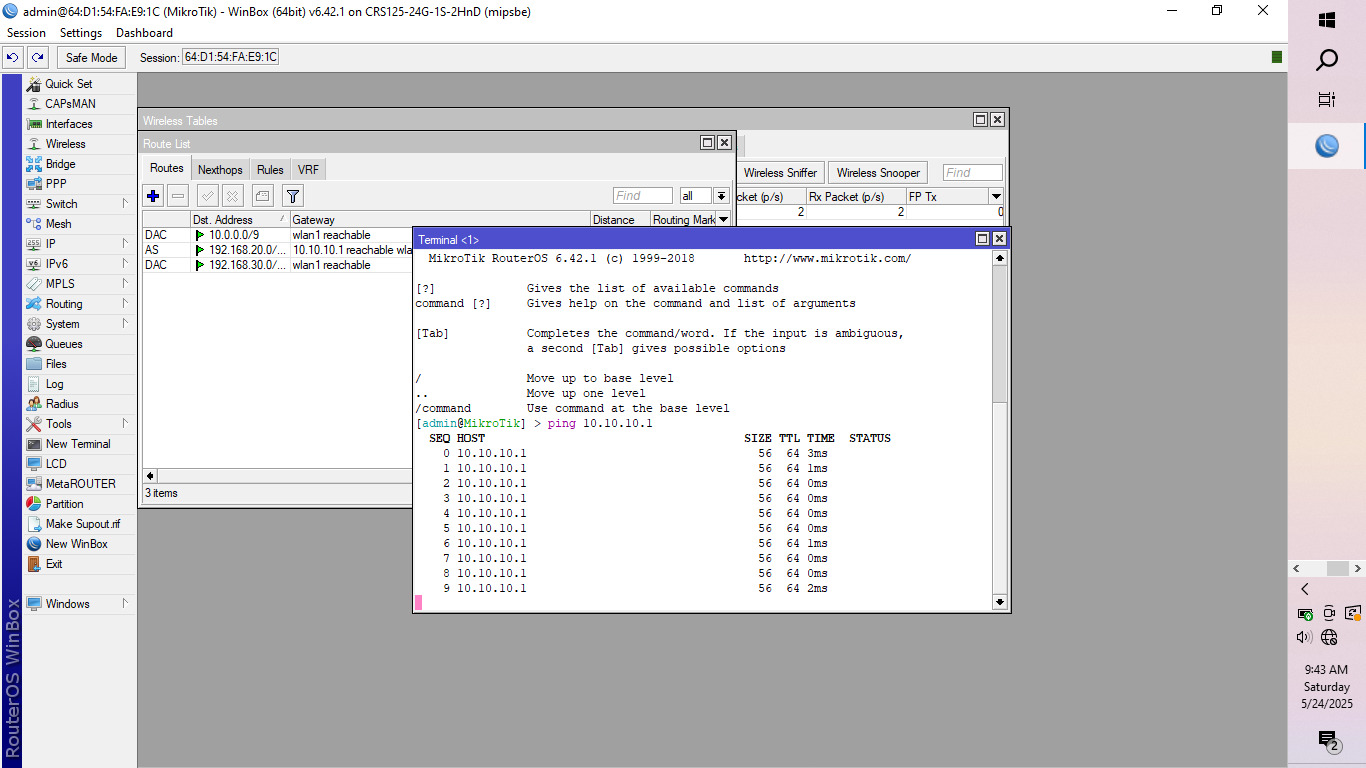
\includegraphics[width=0.5\linewidth]{P1/img/15.jpeg}
        \caption{Lakukan Uji Ping}
        \label{fig:gambar4}
    \end{figure}
\end{enumerate}

\subsection{Wireless Bridge}
\begin{enumerate}
    \item Hubungkan laptop ke masing-masing router melalui kabel LAN dan lakukan reset konfigurasi menggunakan Winbox.
    \begin{figure}[H]
        \centering
        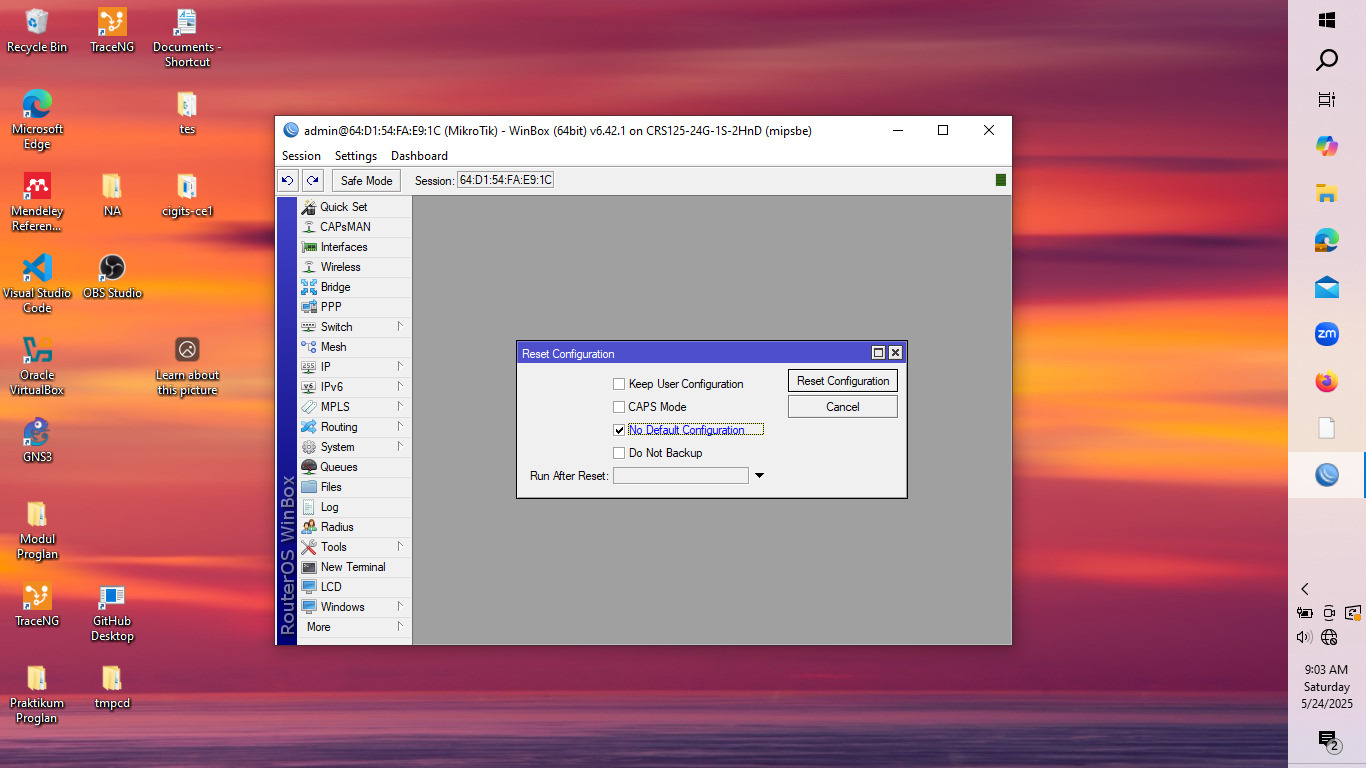
\includegraphics[width=0.5\linewidth]{P1/img/1.jpeg}
        \caption{Reset Configuration}
        \label{fig:gambar4}
    \end{figure}
    \item Aktifkan \texttt{wlan1} pada Router A, atur menjadi mode \textbf{bridge} dan isi SSID dengan \texttt{WirelessBridge\_16}.
    \begin{figure}[H]
        \centering
        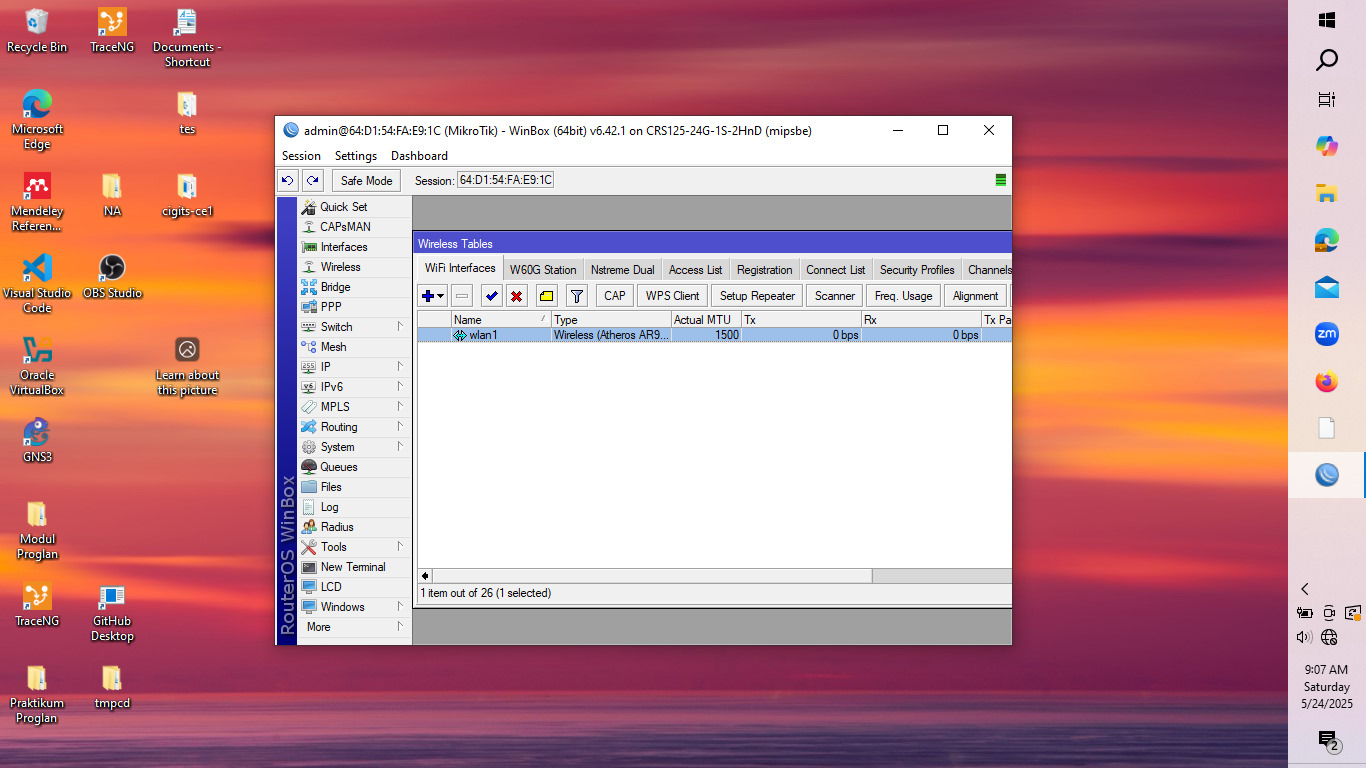
\includegraphics[width=0.5\linewidth]{P1/img/3.jpeg}
        \caption{Aktifkan interface}
        \label{fig:gambar4}
    \end{figure}
    \item Pada Router B, aktifkan \texttt{wlan1}, ubah modenya menjadi \textbf{station pseudobridge}, lalu hubungkan ke SSID dari Router A.
    \begin{figure}[H]
        \centering
        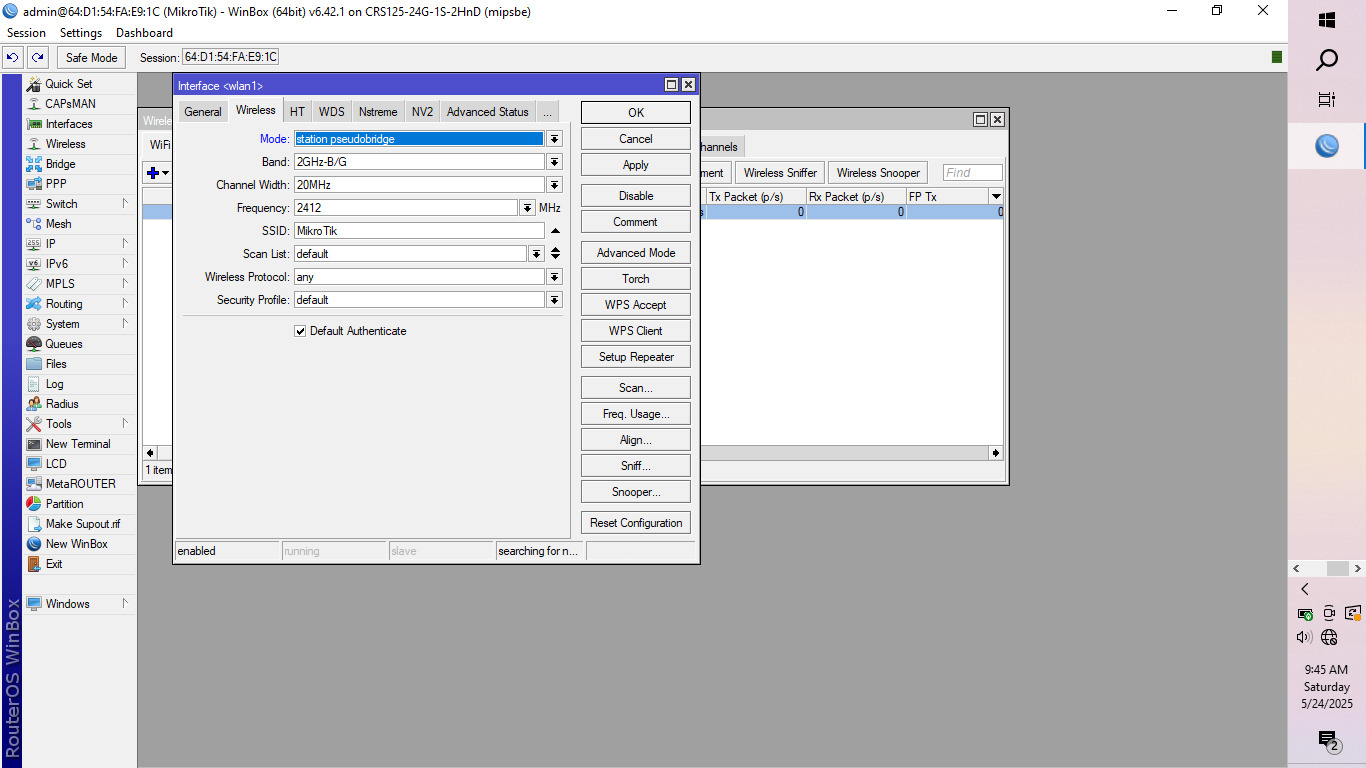
\includegraphics[width=0.5\linewidth]{P1/img/17.jpeg}
        \caption{Aktifkan wlan 1, ubah modenya menjadi Pseudoobrige}
        \label{fig:gambar4}
    \end{figure}
    \item Tambahkan konfigurasi IP pada interface \texttt{wlan1} dan \texttt{ether2} untuk masing-masing router.
    \begin{figure}[H]
        \centering
        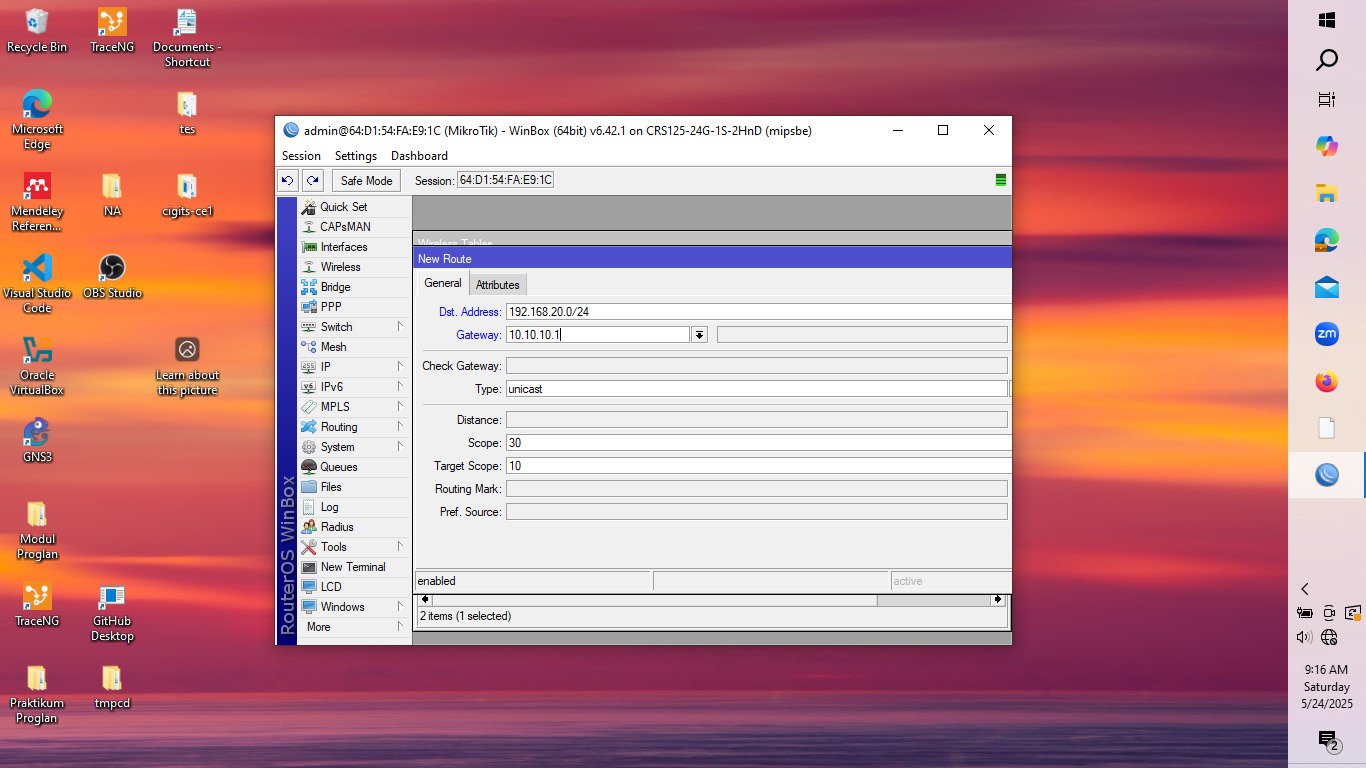
\includegraphics[width=0.5\linewidth]{P1/img/7.jpeg}
        \caption{Konfigurasi Routing}
        \label{fig:gambar4}
    \end{figure}
    \item Buat bridge baru di kedua router dan masukkan interface \texttt{wlan1} dan \texttt{ether2} ke dalam bridge tersebut.
    \begin{figure}[H]
        \centering
        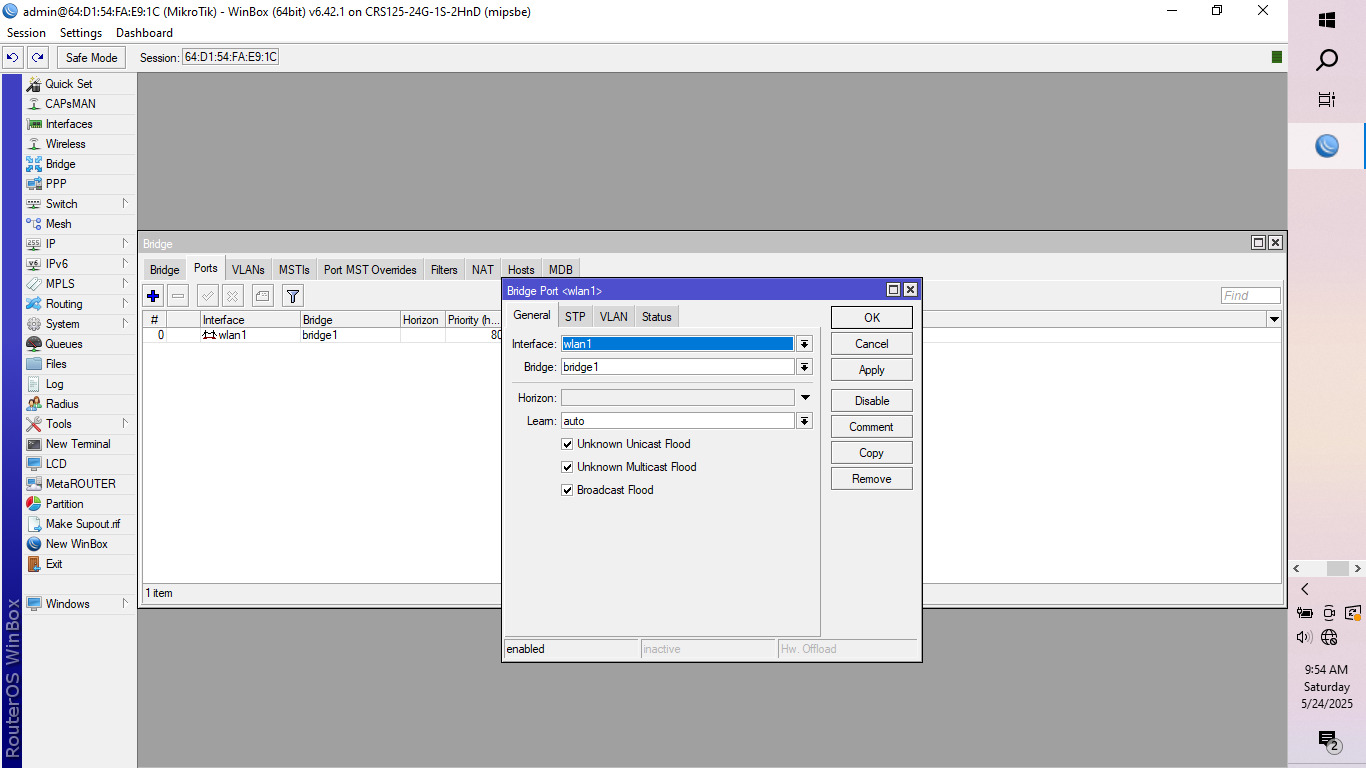
\includegraphics[width=0.5\linewidth]{P1/img/20.jpeg}
        \caption{Buaat bridge baru}
        \label{fig:gambar4}
    \end{figure}
    \item Lakukan \texttt{ping} antar laptop untuk memastikan koneksi berjalan dengan baik.
    \begin{figure}[H]
        \centering
        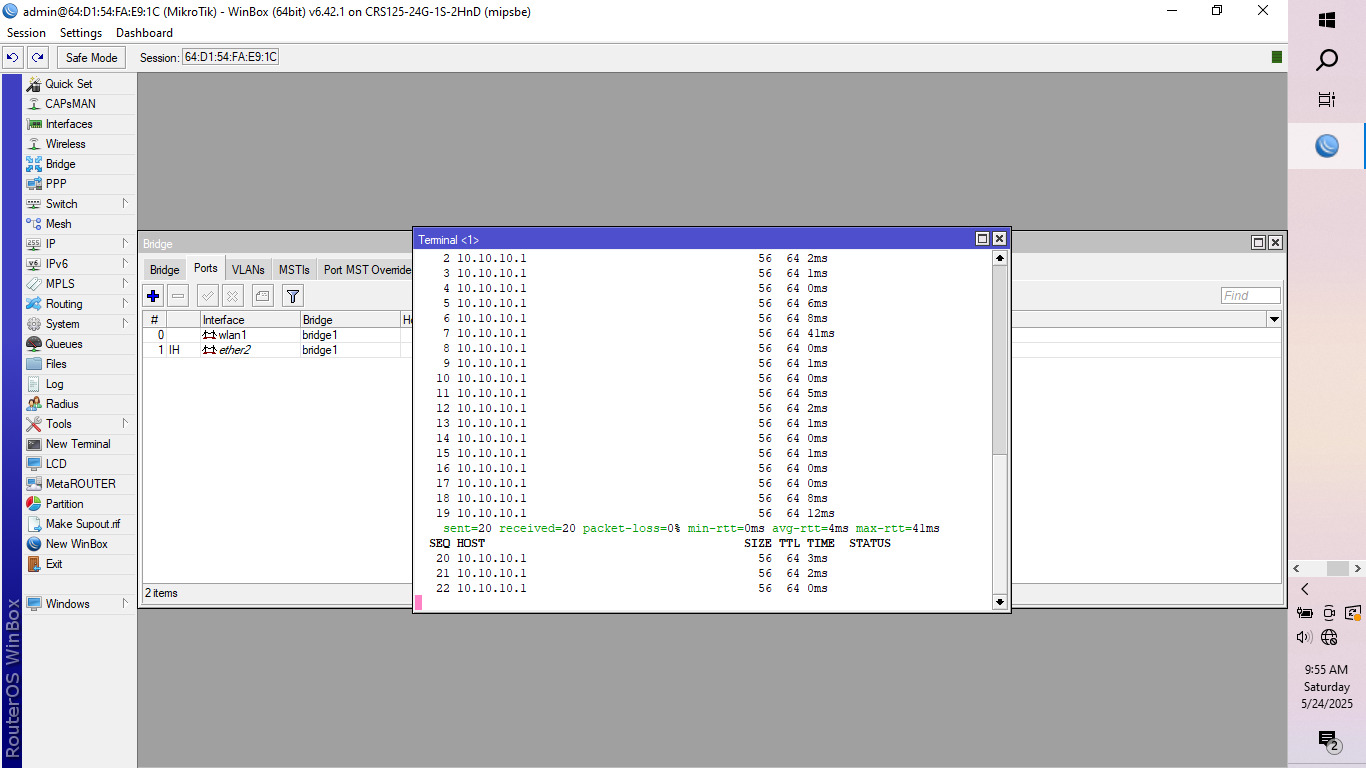
\includegraphics[width=0.5\linewidth]{P1/img/22.jpeg}
        \caption{Lakukan Uji Ping}
        \label{fig:gambar4}
    \end{figure}
\end{enumerate}



\section{Analisis Hasil Percobaan}

Pada praktikum ini dilakukan konfigurasi tiga jenis jaringan nirkabel menggunakan perangkat MikroTik, yaitu Wireless Point to Point, Wireless Point to Multipoint, dan Wireless Bridge. Masing-masing memiliki peran dan keunggulan dalam skenario jaringan yang berbeda-beda.

\\

Konfigurasi ini menghubungkan dua router secara langsung tanpa perantara. Router A berperan sebagai pemancar sinyal (mode \textit{bridge}), sementara Router B menjadi penerima (mode \textit{station}) dengan SSID yang telah disamakan. Setelah pengaturan IP statis dan rute manual disesuaikan, pengujian koneksi dilakukan menggunakan perintah \texttt{ping} antar perangkat. Hasilnya menunjukkan bahwa komunikasi antara dua titik berjalan lancar tanpa kehilangan paket dan dengan waktu respons yang singkat. Topologi ini ideal digunakan untuk menghubungkan dua lokasi tetap yang berjarak jauh secara efisien dan stabil.

\\

Pada skenario ini, satu router dikonfigurasi sebagai pusat koneksi (mode \textit{AP bridge}), sedangkan router lainnya sebagai client (\textit{station bridge}). Dengan SSID yang sama, router client dapat bergabung ke jaringan pusat. Setelah konfigurasi IP dan routing selesai, konektivitas diuji antar laptop yang terhubung. Koneksi berhasil terjalin dan menunjukkan bahwa model ini mampu melayani lebih dari satu perangkat sekaligus. Meskipun fleksibel untuk memperluas jangkauan jaringan, performa jaringan dalam topologi ini cenderung menurun seiring bertambahnya jumlah perangkat yang terhubung karena bandwidth harus dibagi.

\\

Konfigurasi ini ditujukan untuk menyatukan dua jaringan lokal (LAN) menggunakan koneksi nirkabel. Router A diatur sebagai \textit{bridge} seperti sebelumnya, namun Router B menggunakan mode \textit{station pseudobridge}. Setelah membuat interface bridge dan menambahkan \texttt{wlan1} serta \texttt{ether2} ke dalamnya, koneksi antar router dan perangkat berhasil dibangun. Hasil uji ping menunjukkan komunikasi dua arah berjalan tanpa hambatan. Namun, perlu dicatat bahwa mode \textit{pseudobridge} memiliki keterbatasan dalam meneruskan beberapa jenis paket, terutama broadcast atau multicast, sehingga penggunaannya lebih tepat untuk skenario kecil atau jaringan yang tidak memerlukan komunikasi layer 2 penuh.

\section{Hasil Tugas Modul}
\begin{enumerate}
    \item Simulasikan jaringan wireless antara tiga gedung: Gedung Pusat Gedung Lab Gedung Asrama (Hubungkan dua bagian dalam Gedung Asrama (Blok A dan Blok B) menggunakan Wireless Bridge Point-to-Point.)
Menggunakan Point-to-Multipoint (PTMP) di Cisco Packet Tracer.
    \begin{figure}[H]
        \centering
        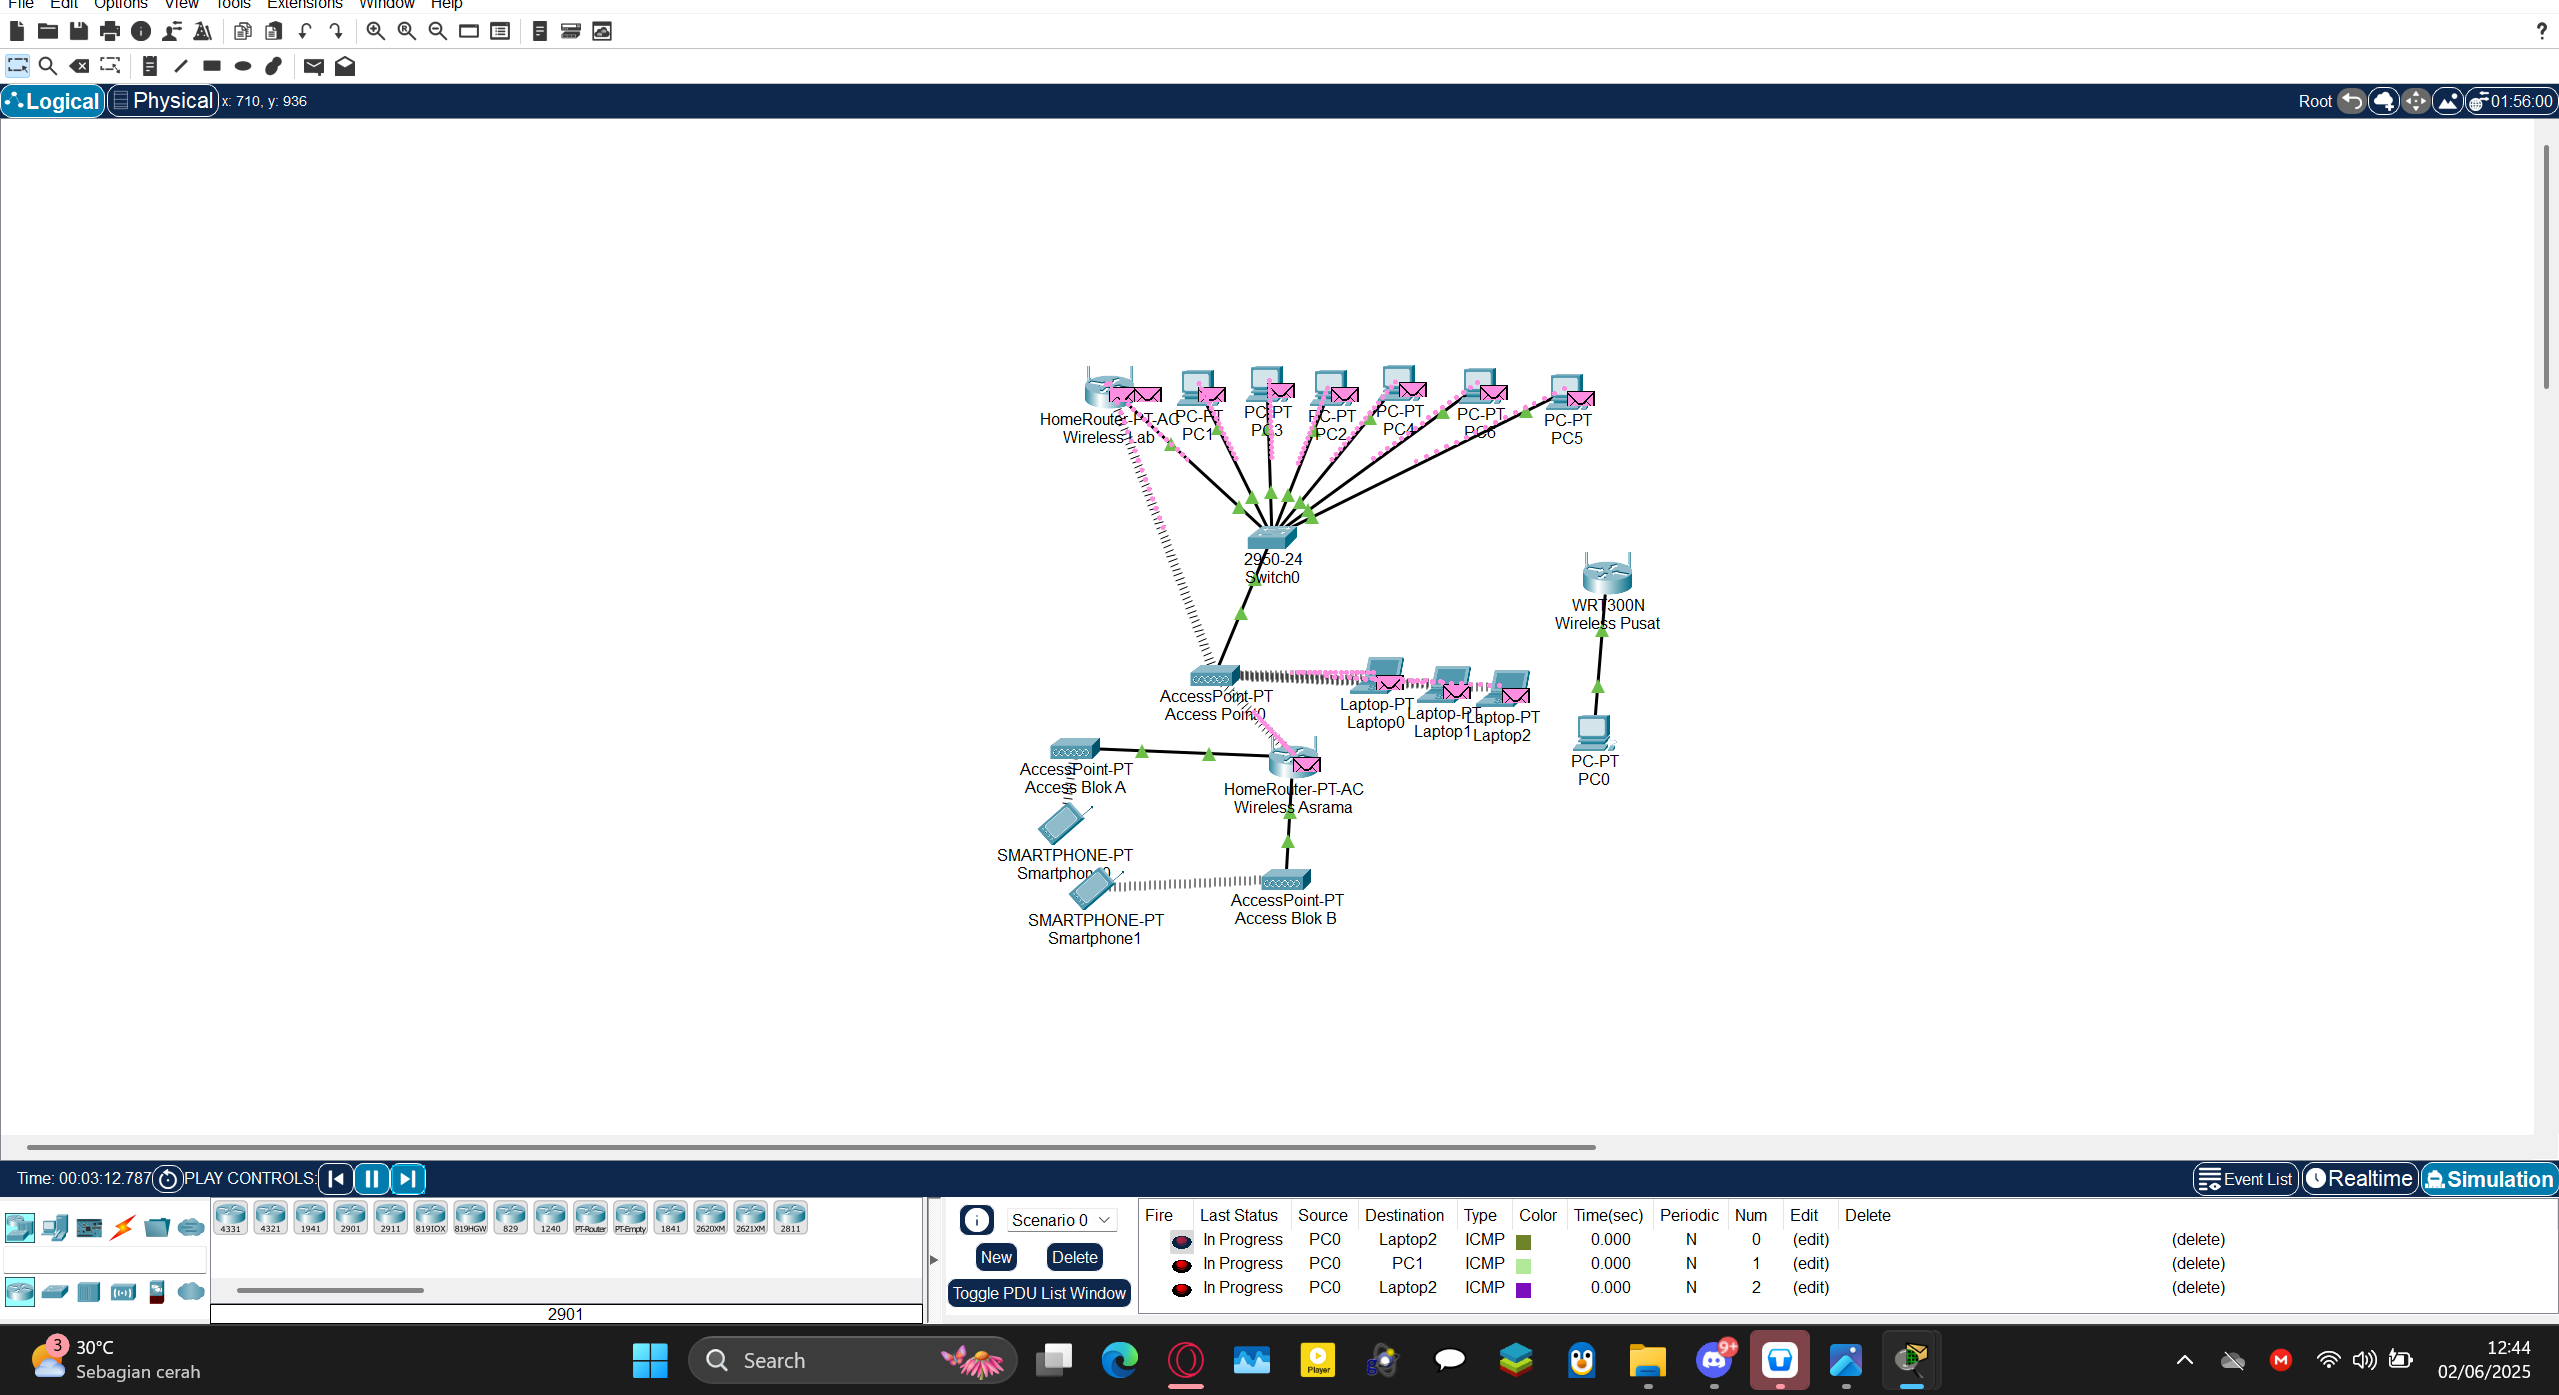
\includegraphics[width=0.8\linewidth]{P1/img/1.png}
        \caption{Dinamis}
        \label{fig:gambar4}
    \end{figure}
Tugas simulasi ini bertujuan untuk membangun jaringan wireless antara tiga gedung, yaitu Gedung Pusat, Gedung Lab, dan Gedung Asrama, dengan menggunakan topologi Point-to-Multipoint (PTMP) di Cisco Packet Tracer. Dalam simulasi ini, Gedung Pusat berperan sebagai access point utama (AP) yang memancarkan sinyal ke client wireless di Gedung Lab dan Gedung Asrama. Khusus untuk Gedung Asrama, terdapat dua bagian, yaitu Blok A dan Blok B, yang dihubungkan secara langsung menggunakan konfigurasi Wireless Bridge Point-to-Point untuk membentuk satu jaringan lokal antar kedua blok. Tujuan dari konfigurasi ini adalah memastikan konektivitas antar gedung dapat tercapai tanpa kabel, serta memungkinkan pertukaran data antar perangkat di seluruh area dengan efisien.
  

\end{enumerate}

\section{Kesimpulan}
Berdasarkan praktikum yang telah dilakukan, dapat disimpulkan bahwa setiap jenis konfigurasi jaringan nirkabel memiliki karakteristik dan fungsi yang berbeda sesuai dengan kebutuhan jaringan yang diinginkan.

Konfigurasi Wireless Point to Point menunjukkan performa terbaik dari segi kestabilan koneksi karena hanya melibatkan dua perangkat yang saling terhubung secara langsung. Sementara itu, pada konfigurasi Wireless Point to Multipoint, sistem lebih fleksibel dan mampu melayani banyak perangkat sekaligus, namun memerlukan manajemen bandwidth yang lebih cermat agar tidak terjadi penurunan performa.

Adapun konfigurasi Wireless Bridge mampu menghubungkan dua jaringan lokal secara nirkabel dan memungkinkan komunikasi antar segmen jaringan, meskipun dengan keterbatasan tertentu seperti dukungan terbatas terhadap paket broadcast atau multicast.

Dengan demikian, pemilihan topologi dan mode konfigurasi harus disesuaikan dengan kebutuhan jaringan yang hendak dibangun, baik dari segi jumlah perangkat, jenis trafik, hingga efisiensi koneksi yang diharapkan.


\section{Lampiran}
\subsection{Dokumentasi saat praktikum}
\begin{figure}[H]
        \centering
        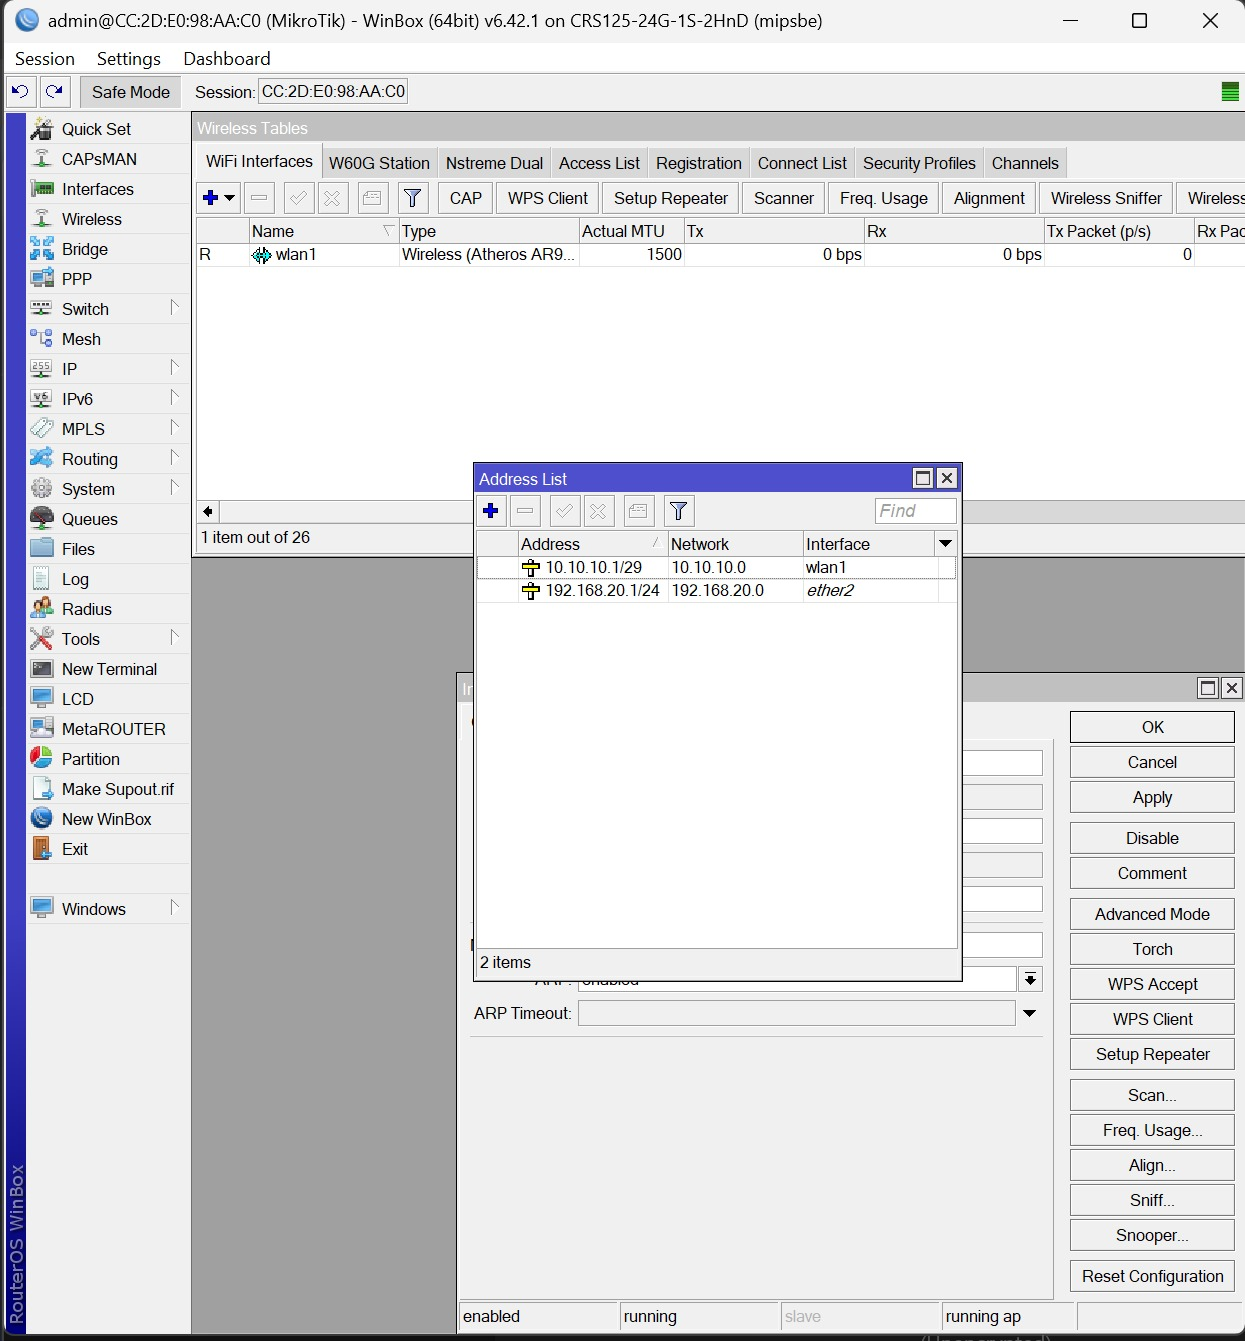
\includegraphics[width=0.5\linewidth]{P1/img/23.jpeg}
        \caption{Dokumentasi}
        \label{fig:gambar1}
    \end{figure}

    \begin{figure}[H]
        \centering
        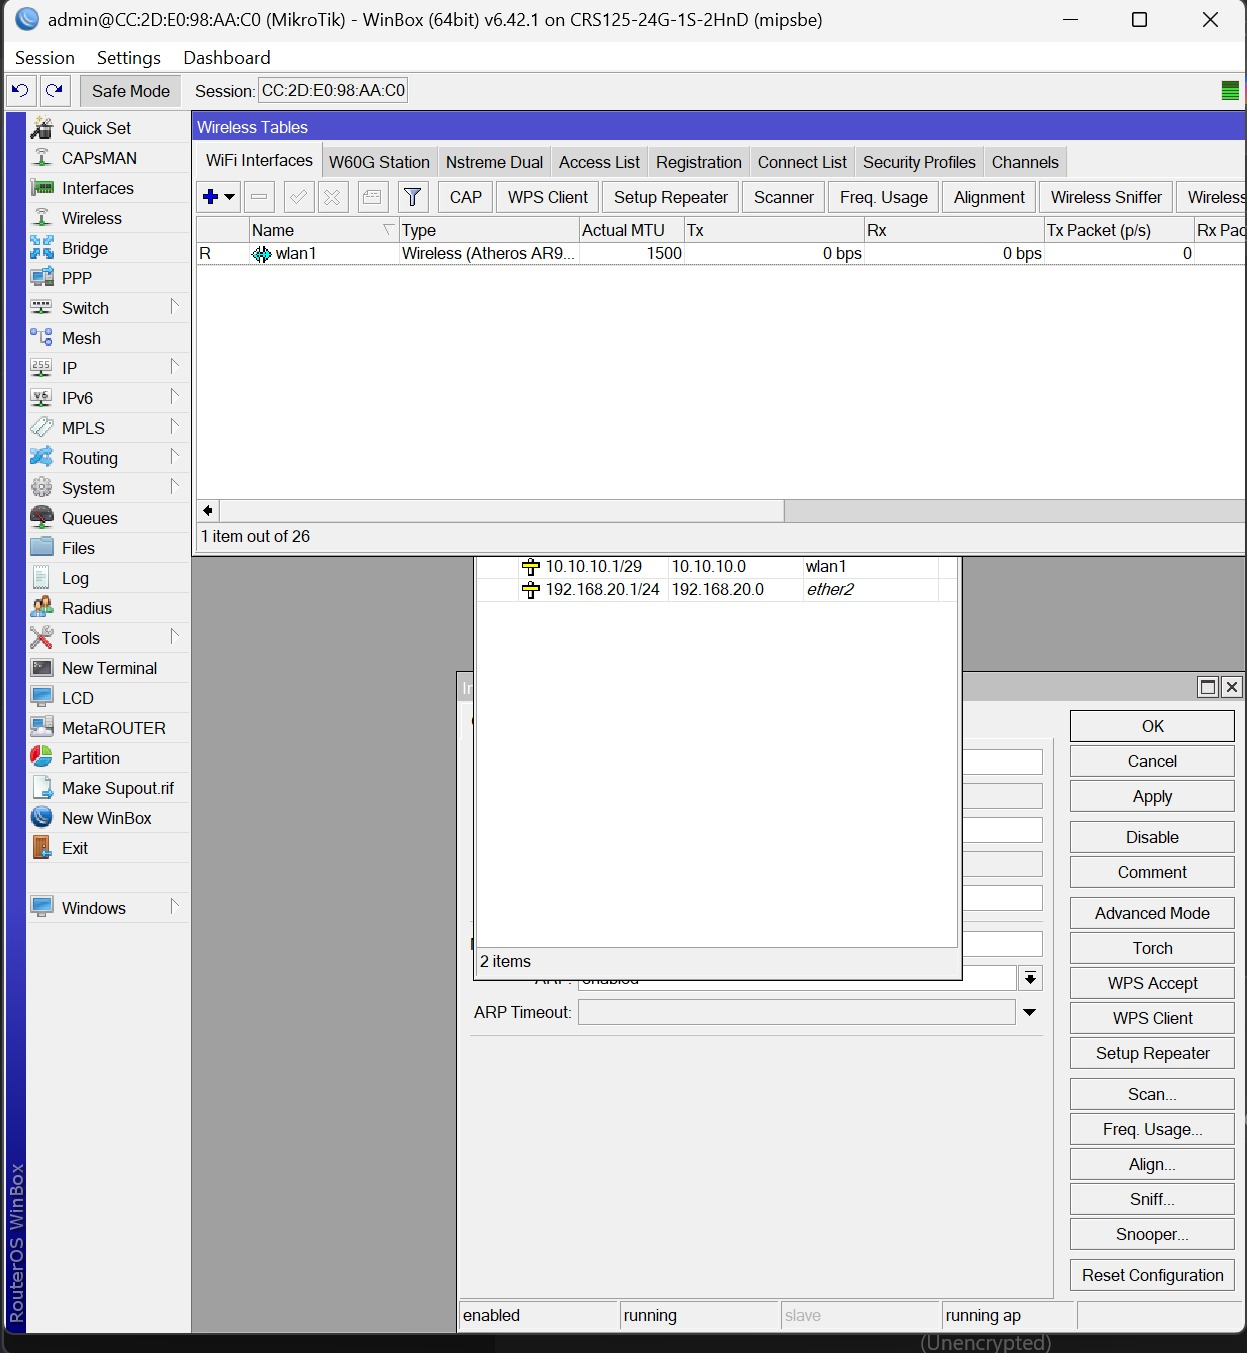
\includegraphics[width=0.5\linewidth]{P1/img/24.jpeg}
        \caption{Dokumentasi}
        \label{fig:gambar1}
    \end{figure}

    \begin{figure}[H]
        \centering
        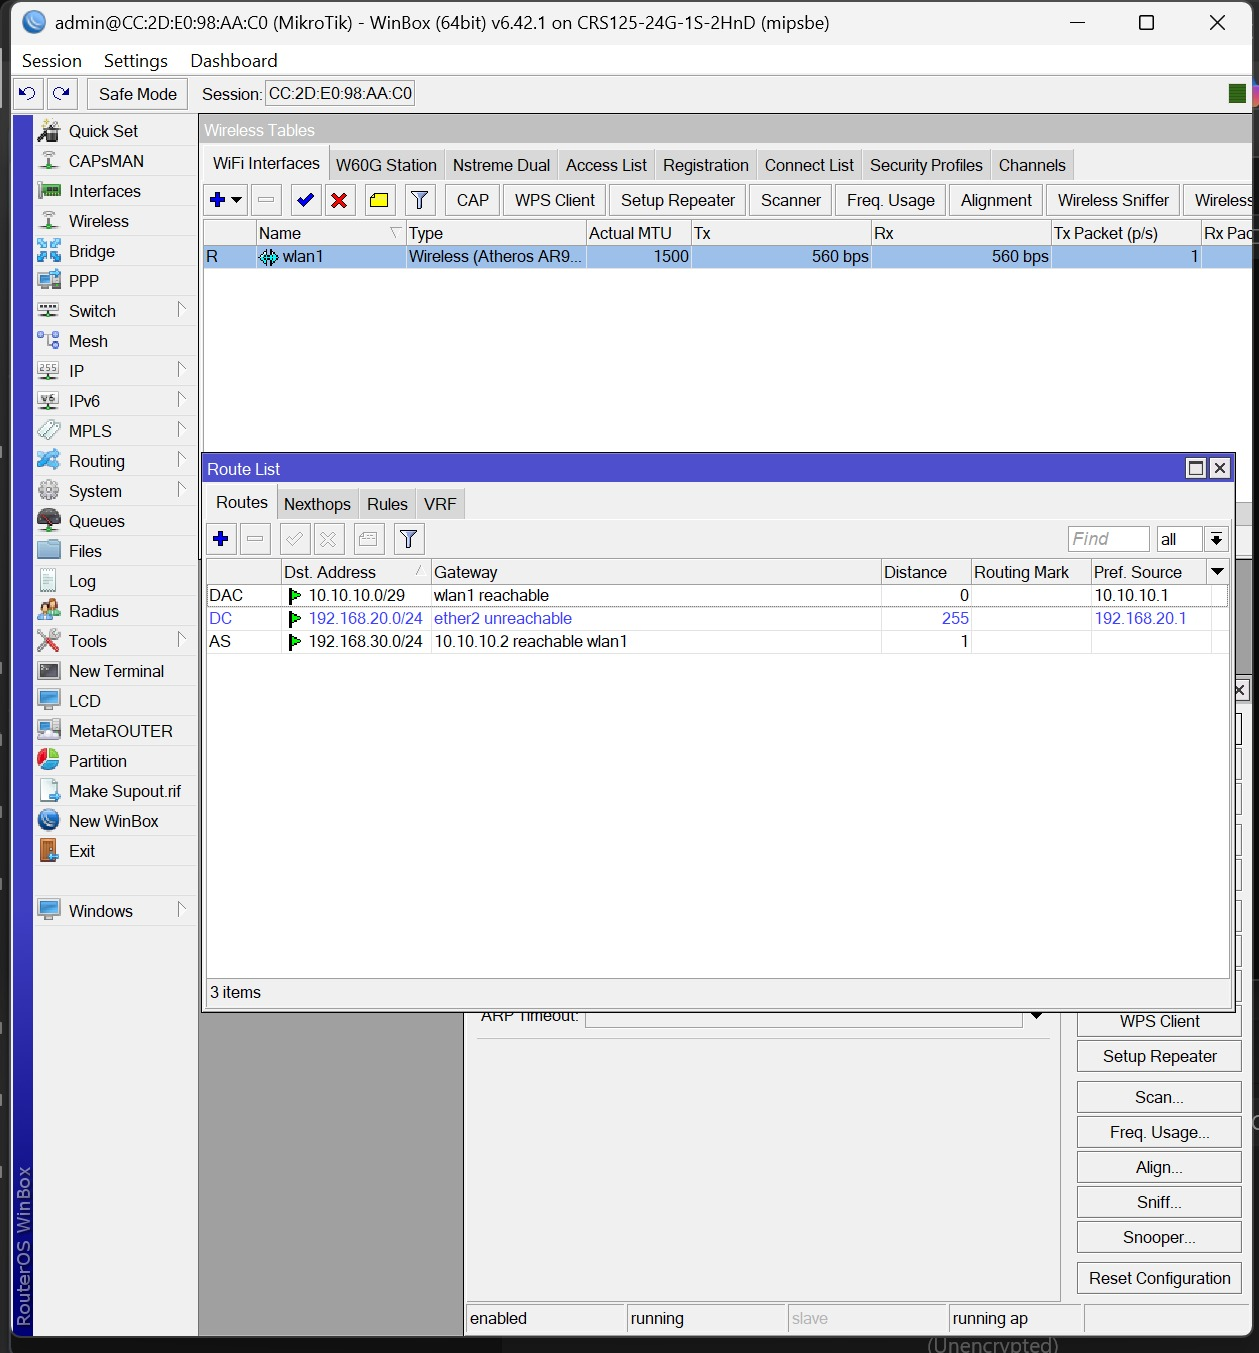
\includegraphics[width=0.5\linewidth]{P1/img/25.jpeg}
        \caption{Dokumentasi}
        \label{fig:gambar1}
    \end{figure}

